\Titelbanner{2}{Lineare Gleichungssysteme}

\paragraph{Tafelbeispiel:} $\displaystyle \frac{10(x+y) + 3}{x-2y+4} = 1, \quad \frac{36x-3y}{7(x-y)+3} = 3$
\begin{enumerate}
    \item Sortieren nach $x$ und $y$ 
    \begin{align*}
        9x +12 y &= 1 \quad (1) \\
        15x+18y &= 9 \quad (2)
    \end{align*}
    \item Prüfe auf lineare Unabhängigkeit, d.\,h. Berechne $a_1 b_2 - a_2 b_1$ (Determinante, vgl. Vorlesung): 
    \begin{align*}       
        9\cdot 18 - 15\cdot 12 = 162-180 \neq 0 \quad \Rightarrow \qq{genau ein Lösungspaar ($x,y$)}
    \end{align*}      
    \item Lösen, bspw. durch geschickte Linearkombination (Elimination von $y$)
    \begin{align*}
        2\cdot (2) - 3\cdot (1): \quad \hp{1}3x &= \hp{-}15 \quad \Rightarrow x=5 \\
        \qq{in} (1): \quad 12y &= -44 \quad \Rightarrow y = -\frac{11}{3} \\
        \Rightarrow \qq{Lösungsmenge} \mathbb{L} &= \uuline{\Bigg\{\qty(5;-\frac{11}{3})\Bigg\}}
    \end{align*}
\end{enumerate}

\paragraph{Aufgabe 1: } \emph{Zwei lineare Gleichungen mit zwei Unbekannten} \hfill Ziel (a) bis (d)\\[0.2cm]
\begin{enumerate}[label=(\alph*)]
    \item $~$\\[-1.45 cm]\begin{align*}
        &33x+12y=25 \quad (1) \\ 
        &11x-\hp{1}3y=\hp{2}6 \quad (2) \\
        &(1) - 3\cdot (2): \quad 21y = 7 \quad\Rightarrow \quad y = \frac{1}{3}, \qq{in (2):} x = \frac{7}{11} \qquad \Rightarrow \qquad \uuline{\mathbb{L} = \Bigg\{\qty(\frac{7}{11};\frac{1}{3})\Bigg\}}
    \end{align*}
    \item $~$\\[-1.45cm] 
    \begin{align*}
        &\begin{rcases}
            \frac{2x + 3y}{3x-y} = \frac{17}{9} \\
            \dfrac{3x+4y}{6x-1}=2
        \end{rcases} \quad \Longrightarrow \quad 
        \begin{array}{l}
            3x-4y = 0 \quad (1) \\
            9x -4y = 2 \quad (2)
        \end{array} \\
        &\hp{3\cdot}\;\,(1) -(2): \quad 6x = 2 \quad\Rightarrow\quad x = \frac{1}{3}\\
        &3\cdot(1) -(2): \quad 8y = 2 \quad\Rightarrow\quad y = \frac{1}{4} \qquad \Rightarrow \qquad \uuline{\mathbb{L} = \Bigg\{\qty(\frac{1}{3};\frac{1}{4})\Bigg\}}
    \end{align*}
    \item $~$\\[-1.45cm] 
    \begin{align*}
        &\begin{rcases}
            \frac{x+2}{y+3}=\frac{1}{3} \\
            \frac{y+3}{2y-5x}=\frac{3}{5}
        \end{rcases} \quad \Longrightarrow \quad 
        \begin{array}{l}
            \hp{1}3x-y = \;\;\;-3 \quad (1) \\
            15x -y = -15 \quad (2)
        \end{array} \\
        &(1) - (2): \quad -12x = 12 \quad \Rightarrow \quad  x = -1\\
        &\quad\,\text{in } (1): \quad \hp{-12x = 12\quad \Rightarrow \quad} \,y = 0 \qquad \Longrightarrow \qquad \uuline{\mathbb{L} = \big\{\qty(-1;0)\big\}}
    \end{align*}
    \item $~$\\[-1.45cm] 
    \begin{align*}
        &ax+by=2a \quad (1)\\
        &\frac{x}{b}-\frac{y}{a}=\frac{2}{a} \quad (2)\\
        &(1) - ab \cdot (2): \;\;\,\cancel{2}by = \cancel{2}(a-b) \quad \Rightarrow \quad y = \frac{a}{b}-1 \\
        &\hp{(1)-}\text{in } (1): \quad ax + \cancel{a} -b = \cancel{2}a \quad \Rightarrow \quad x=\frac{b}{a}+ 1 \qquad \Longrightarrow \qquad \uuline{\mathbb{L} = \Bigg\{\qty(\frac{b}{a}+1;\frac{a}{b}-1)\Bigg\}}
    \end{align*}
    \item $~$\\[-1.45cm] 
    \begin{alignat*}{2}
        &x+14y=\frac{1}{\sqrt{2}}-7\sqrt{2} \;\;\;\quad (1)\\
        &3\sqrt{2}x-\frac{y}{\sqrt{3}}=3+\frac{1}{\sqrt{6}} \quad (2)\\
        &(1) - \frac{1}{3\sqrt{2}}\cdot (2): \quad\cancel{\qty(14+\frac{1}{3\sqrt{6}})}y &&= \bcancel{\frac{1}{\sqrt{2}}} - 7\sqrt{2} - \bcancel{\frac{1}{\sqrt{2}}} - \frac{1}{3\sqrt{12}} \\
        & &&= -\frac{1}{\sqrt{2}} \cancel{\qty(14+\frac{1}{3\sqrt{6}})} \quad \Rightarrow \quad y = -\frac{1}{\sqrt{2}} \\
        & \text{in } (1): \quad x-\cancel{7\sqrt{2}} = \frac{1}{\sqrt{2}} - \cancel{7\sqrt{2}} \quad &&\Rightarrow \quad x = \frac{1}{\sqrt{2}} \qquad \Longrightarrow \qquad \uuline{\mathbb{L} = \Bigg\{\qty(\frac{1}{\sqrt{2}};-\frac{1}{\sqrt{2}})\Bigg\}}
    \end{alignat*}
    \item $~$\\[-1.45cm] 
    \begin{alignat*}{3}
        &\frac{x}{a+b}+\frac{y}{a-b}=a+b \quad (1)\\
        &\frac{x}{a}-\frac{y}{b}=2b \hspace{1.68cm}\quad (2) \\
        &(a+b) \cdot (1) - a\cdot(2): \quad \qty(\frac{a+b}{a-b}+\frac{a}{b}) y &&= a^2 +b^2 \\
        && \hspace{-3.5cm}\bcancel{\qty(\cancel{ab}+b^2 + a^2 - \cancel{ab})}y &= b(a-b)(a^2 +b^2) \\
        && \hspace{-1cm}\Rightarrow y &= b(a-b) \\
        &\text{in }(1): \quad \frac{x}{a+b} +\cancel{b} = a+ \cancel{b} & \hspace{-1cm}\Rightarrow x &= a(a+b) \quad \Longrightarrow \quad \uuline{\mathbb{L} = \big\{\qty(a(a+b);b(a-b))\big\}}
    \end{alignat*}
    \item $~$\\[-1.45cm] 
    \begin{alignat*}{3}
        &39x-38y=1 \quad (1) \\
        &91x-57y=4 \quad (2) \\
        &2\cdot(2)-3\cdot(1): \quad (182-117)x = 5 \quad &&\Rightarrow \quad x = \frac{1}{13} \\
        &\text{in } (1): \quad 38y = 2 &&  \Rightarrow \quad y = \frac{1}{19} \qquad \Longrightarrow \qquad \uuline{\mathbb{L} = \Bigg\{\qty(\frac{1}{13};\frac{1}{19})\Bigg\}}
    \end{alignat*}
\end{enumerate}

\newpage
\paragraph{Aufgabe 2: } \emph{Drei Gleichungen mit drei Unbekannten} \hfill Ziel: (a) und (b)\\[0.2cm]
%
\emph{Tafelbeispiel: }
\begin{alignat*}{2}
    x+ \hp{2}y + \hp{4}z &= 9 &&\quad (1) \\
    x+2y+4z&=15 &&\quad (2) \\
    x+3x+9z&=23 &&\quad (3)
\end{alignat*}
Vorgehen: Wir wollen eine Linearkombination der drei Gleichungen finden, sodass (bspw.) $x$ und $y$ verschwinden; d.\,h. in $a\cdot(1)+b\cdot(2)+c\cdot(3)$ soll $a+b+c =0$ sein und $a+2b+3c=0$. Wir haben offenbar die Freiheit, $a=1$ zu wählen, also $b=-2$ und $c=1$.
\begin{align*}
    &(1)-2\cdot(2)+(3): \quad 2z=2 \quad \Rightarrow \quad z=1 \\
    &\text{in }(1): \quad x+\hp{2}y = 8\;\;\; \quad(4)\\
    &\text{in }(2): \quad x+2y = 11 \quad (5)
\end{align*}
Die Gleichungen (4),(5) können nun mit den früheren Methoden gelöst werden. \\
Optionale Kreativlösung: Angenommen $x,y \in \mathbb{N}$. Nach (5) muss $x$ ungerade sein, damit nach (4) auch $y$. Die einzigen positiven Zerlegungen der Zahl 8 in zwei ungerade Zahlen sind (1,7) und (3,5). Nur letztere löst (4) und (5). Wir erhalten $\uuline{\mathbb{L} = \{(5;3;1)\}}$.

\emph{Lösung:}

\begin{enumerate}[label=(\alph*)]
    \item $~$\\[-1.45 cm]
    \begin{align*}
        &\hp{3}x-\hp{5}y+5z=5 \quad (1)\\
        &3x+7y-5z=5\quad (2)\\
        &\hp{3}x+\hp{5}y-\hp{5}z=1 \quad (3) \\
        &2\cdot(1) + (2) - 5\cdot(3): \quad 10z=10 \quad \Rightarrow \quad z=1 \\
        &\begin{rcases}
        \text{in }(1): \quad x-y = 0\\
        \text{in }(3): \quad x+y = 2
        \end{rcases} \quad x=y=1 \qquad \Longrightarrow \qquad \uuline{\mathbb{L} = \big\{\qty(1;1;1)\big\}}
    \end{align*}
    \item $~$\\[-1.45cm] 
    \begin{align*}
        &3x-4y+3z=\hp{-}4\quad (1)\\
        &\minus x+\hp{4}y-\hp{5}z=-2\quad (2)\\
        &7x+4y-5z=\hp{-}0 \quad (3) \\
        &(1) + 8\cdot (2) -(3): \quad -12x = -12 \quad \Rightarrow \quad x=1 \\
        &\begin{rcases}
            \text{in }(1): \quad -4y+3z = \hp{-}1\\
            \text{in }(2): \quad \hp{-4}y-z = -1
            \end{rcases} \quad y=2, z=3 \qquad \Longrightarrow \qquad \uuline{\mathbb{L} = \big\{\qty(1;2;3)\big\}}
    \end{align*}
    \item $~$\\[-1.45cm] 
    \begin{align*}
        &x+y=b+a\quad (1)\\
        &x+z=a+c\quad (2) \qquad \text{Lösung durch Draufschauen.}\\
        &y+z=c+b\quad (3)\\
        &(1)+(2)-(3): \quad 2x=2a \\
        &(1)-(2)+(3): \quad 2y=2b \\
        &(2)+(3)-(1): \quad 2z=2c \qquad \Longrightarrow \qquad \uuline{\mathbb{L} = \big\{\qty(a;b;c)\big\}}
    \end{align*}
    \newpage
    \item $~$\\[-1.45cm] 
    \begin{align*}
        &\hp{\minus}6x-4y+\;\;\;\;8z=0\quad (1) \\
        &\minus2x+\hp{4}y-\,\hp{11}z=0\quad (2) \qquad \text{Da $(1)-3\cdot(2)=(3)$, ist das System unterbestimmt.}\\
        &12x-7y+11z=0\quad(3)\\
        &(1)+3\cdot(2): \quad -\hp{2}y+5z = 0 \quad \Rightarrow y=5z \\
        &(1)+4\cdot(2): \quad -2x+4z=0 \quad \Rightarrow x=2z \qquad \Longrightarrow \qquad \uuline{\mathbb{L} = \big\{\qty(2z;5z;z)\mid z\in\mathbb{R}\big\}
        }
    \end{align*}
\end{enumerate}

% 
\textbf{Aufgabe 3: } \emph{Parametrisierung von Lösungsmengen}\\[0.2cm]
Geben Sie die Lösungsmenge der Gleichung $13x-7y=1$ an für
\begin{align*}
&\text{(a) } \hspace{0.2cm} x,y\in\mathbb{R}\,;\\[0.2cm]
&\text{(b) } \hspace{0.2cm} x,y\in\mathbb{N}\,.
\end{align*}
(a) Für $x,y \in \mathbb{R}$ ist nichts zu beachten. Wir Lösen die Gleichung nach $x$ auf und erhalten 
\begin{align*}
    x = \frac{1+7y}{13} \qquad \Longrightarrow \qquad \uuline{\mathbb{L} = \Bigg\{\qty(\frac{1+7\lambda}{13};\lambda)\mid \lambda \in\mathbb{R}\Bigg\}}.
\end{align*}
(b) Für $x,y \in \mathbb{N}$ muss $1+7n, n\in\mathbb{N}$, ein Vielfaches von 13 sein. Die kleinste natürliche Zahl, für die das gilt, ist $n=11$ (ausprobieren), d.\,h. alle übrigen Teiler liegen in 13er-Schritten darüber.
\begin{table}[htp]
    \centering
    \begin{tabular}{l r r r r r r r r r r r r}
        \toprule 
        $n$ & 1 & 2 & 3 & 4 & 5 & 6 & 7 & 8 & 9 & 10 & 11\\
        \midrule
        $7n+1$ & 8 & 15 & 22 & 29 & 36 & 43 & 50 & 57 & 64 & 71 & 78 \\
        13-Reihe & 13 & 26 & 39 & 52 & 65 & 78 
    \end{tabular}
\end{table}

Setzen wir also $\lambda = 11+13n$ in $\mathbb{L}$ von oben ein, ergibt sich $\uuline{\mathbb{L} = \Bigg\{\qty(6+7n;11+13n)\mid n \in\mathbb{N}_0\Bigg\}}$.

\paragraph{Aufgabe 4: } \emph{Gleichungssysteme} \hfill Ziel (a) und (b)\\[0.2cm]

\emph{Tafelbeispiel:} In dieser Aufgabe werden nicht linear aussehende Gleichungen auf lineare Gleichungssysteme zurückgeführt. 
\begin{alignat*}{2}
    (1-x)^2 &= 5y^2 - 4(x-2)^2 \quad &&(1) \\
    2(x^2-y^2) &= 6x-5 &&(2).
\end{alignat*}
Sortieren wir das Gleichungssystem um, ergibt sich 
\begin{alignat*}{2}
    &5(x^2-y^2)-18x + 17 = 0 \quad (3)\\
    &2(x^2-y^2)-\hp{1}6x + \hp{1}5 = 0 \quad (4)\\
    &(3)-\frac{5}{2}\cdot(2): \quad -3x + \frac{9}{2} = 0 \quad\Rightarrow \quad &&x=\frac{3}{2} \\
    &\text{in }(2): \quad y^2 =x^2 -3x + \frac{5}{2} = \frac{1}{4} \quad &&y= \pm \frac{1}{2} \qquad \Longrightarrow \qquad \uuline{\mathbb{L} = \Bigg\{\qty(\frac{1}{2};\pm \frac{1}{2})\Bigg\}}. 
\end{alignat*}

\emph{Lösung:}

\begin{enumerate}[label=(\alph*)]
    \item $~$\\[-1.45 cm]
    \begin{align*}
        &x^2+y^2=2(xy+2) \quad(1) \quad \Rightarrow \quad (x-y)^2 = 4 \Rightarrow x-y = \pm 2 \quad (1a)\\
        &x\hp{^2}+y\hp{^2} =6 \hp{(xy+2)} \quad(2)\\
        &(1a)+(2): \quad 2x = \begin{cases}
            8, & \text{oberes VZ} \\
            4, & \text{unteres VZ}
        \end{cases}\\
        &\text{in }(2): \qquad\quad\; y = \begin{cases}
            2, & \text{oberes VZ} \\
            4, & \text{unteres VZ}
        \end{cases} \qquad \Longrightarrow \qquad \uuline{\mathbb{L} = \Bigg\{\qty(4;2),(2;4)\Bigg\}}
    \end{align*}
    \item $~$\\[-1.45cm]
    \begin{align*}
        &\frac{12}{\sqrt{x-1}}+\frac{5}{\sqrt{y+\frac{1}{4}}}=5\quad (1)\\ 
        &\frac{8}{\sqrt{x-1}}+\frac{10}{\sqrt{y+\frac{1}{4}}}=6\quad(2)\\
        &2\cdot(1)-(2):\hp{3\cdot}\; \quad 16 = 4\sqrt{x-1}\;\;\; \quad \Rightarrow \quad x=17 \\
        &2\cdot(1)-3\cdot(2): \quad 20 = 8\sqrt{y+\frac{1}{4}} \quad \Rightarrow \quad y=6 \qquad \Longrightarrow \qquad \uuline{\mathbb{L} = \Bigg\{\qty(17;6)\Bigg\}}
    \end{align*} 
    Optionaler Hinweis: nicht immer muss alles mühsam quadriert und aufgelöst werden, sondern man kann auch versuchen draufzuschauen. 
    \begin{itemize}
        \item Was ergibt 8 multipliziert mit 20? Antwort: $\textstyle\frac{10}{4}=\frac{5}{2}$
        \item Die Wurzel woraus ist $\textstyle\frac{5}{2}$? Antwort: $\textstyle\frac{25}{4}$. 
        \item Damit ist $y = \frac{25}{4}-\frac{1}{4}= \frac{24}{4} = 6$.
    \end{itemize}
    \vspace{3mm}
    \item $~$\\[-1.45cm]
    \begin{align*}
        &\frac{x^2-y^2}{2x+3}+y^2=(x+y)x-xy \quad \Rightarrow \quad \frac{x^2 -y^2}{2x+3} = x^2 - y^2\quad(1) \\
        &y-2x=3 \quad (2)
    \end{align*}
    \begin{align*}
        \text{Fall } x^2 \neq y^2 \quad
        \begin{rcases}
            (1): 1=2x+3 \quad \Rightarrow x=-1 \\
            \text{in }(2): \quad y=1
        \end{rcases} \text{ Widerspruch}
    \end{align*}
    \begin{align*}
        \text{Fall } x = \pm y \quad (2): \quad y=
        \begin{cases}
            -3, &\text{oberes VZ}\\
            1, &\text{unteres VZ}
        \end{cases} \qquad \Longrightarrow \qquad \uuline{\mathbb{L} = \Bigg\{\qty(-3;-3),(-1;1)\Bigg\}}
    \end{align*}
\end{enumerate}

\newpage
\paragraph{Aufgabe 5: } \emph{Ungleichungssysteme}
\begin{enumerate}[label=(\alph*), labelindent=1em,labelsep=0.5cm]
\item Es ist die Lösungsmenge des folgenden Systems an Ungleichungen zu skizzieren. Welche der Ungleichungen können weggelassen werden, ohne dass sich die Lösungsmenge ändert?

\begin{minipage}{0.2\textwidth}
    \begin{alignat*}{3}
        2x-3y&\geq -6\,,\\
        x-2y&< 11\,,\\
        x&>-y-1\,,\\
        x&<5\,,\\
        x&\geq 0\,,\\
        y&\geq 0
    \end{alignat*}
\end{minipage}
\begin{minipage}{0.8\textwidth}
    \centering
        \begin{tikzpicture}
            \begin{axis}[disabledatascaling, axis lines=middle, xlabel={x}, ylabel={y}, height=7.8cm, domain=-2:10, xmin=-3,xmax=11, ymin=-8, ymax=9, axis equal, legend pos= outer north east]
                \addplot[no marks, black, thick, ]{2/3*x+2};
                \addplot[no marks, FSUblau, thick]{0.5*x-11/2};
                \addplot[no marks, Gruen, thick]{-x-1};
                \draw[thick, PAForange, thick] (5,-8)--(5,8)node[right]{$x<5$};
                \fill[FSUblau, fill opacity =0.3] (0,0)--(5,0) --(5,16/3) -- (0,2) -- cycle;
                \legend{$\textstyle y = \frac{2}{3}x+2$, $\textstyle y = \frac{1}{2}x-\frac{11}{2}$, $\textstyle y = -x-1$};
            \end{axis}
        \end{tikzpicture}
\end{minipage}
Offenbar können die zweite und dritte Gleichung weggelassen werden, ohne dass sich etwas am schraffierten Gebiet ändert. 

\item \textbf{*} Welches Gebiet im ersten Oktanden ($x\ge 0$, $y\ge 0$, $z\ge 0$) wird durch die folgenden Ungleichungen definiert?
\begin{align*}
    x+y&\ge z\,,\\
    x+z&\ge y\,,\\
    y+z&\ge x
\end{align*}

\begin{minipage}{0.4\textwidth}
    Die Ungleichungen beschreiben eine dreiseitige (unendlich große) Pyramide, deren Spitze auf dem Koordinatenursprung liegt und deren Kanten jeweils die $x-y-$, $x-z-$ und $x-z$-Ebene halbieren.
\end{minipage}
\begin{minipage}{0.6\textwidth}
    \centering
        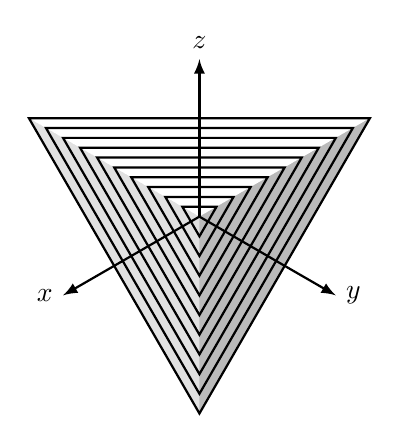
\begin{tikzpicture}
            \draw[thick, -{latex}](0,0) -- (-30:2)node[right]{$y$};
            \draw[thick, -{latex}](0,0) -- (90:2)node[above]{$z$};
            \draw[thick, -{latex}](0,0) -- (210:2)node[left]{$x$};
            \foreach \x in {0.25,0.5,...,2.5}{
                \draw[thick] (-90:\x) -- (30:\x) -- (150:\x) -- cycle;
                \fill[fill opacity=0.01] (0,0) -- (-90:2.5) -- (150:2.5) -- cycle;
                \fill[fill opacity=0.03] (0,0) -- (-90:2.5) -- (30:2.5) -- cycle;
            }
        \end{tikzpicture}
\end{minipage}

\end{enumerate}